\documentclass[25pt, a0paper, landscape, margin=0mm, innermargin=15mm, blockverticalspace=15mm, colspace=15mm, subcolspace=8mm]{tikzposter}

\usepackage{blindtext}
\usepackage{comment}
\usepackage{authblk}
\usetikzlibrary{positioning}
% \geometry{paperwidth=40in,paperheight=50in}
\usetheme{Simple}

\definecolor{habib}{RGB}{92,37,104}
\colorlet{titlebgcolor}{habib}
\colorlet{blocktitlefgcolor}{habib}


% title shit
\definetitlestyle{sampletitle}{
width=750mm, roundedcorners=20, linewidth=0pt, innersep=5pt,
titletotopverticalspace=10mm, titletoblockverticalspace=30mm
}{
\begin{scope}[line width=\titlelinewidth, rounded corners=\titleroundedcorners]
\draw[color=blocktitlebgcolor, fill=titlebgcolor]
(\titleposleft,\titleposbottom) rectangle (\titleposright,\titlepostop);
\end{scope}
}
\usetitlestyle{sampletitle}
\title{{\centering Protien Complex Prediction via Ensemble Clustering}}
\author[1]{Ali Hamza}
\author[1]{M. Usaid Rehman}
\author[1]{Haris K. Ladhani}
\author[1]{Maham S. Patel}
\author[1]{Nadia Nasir}
\author[2]{Humaira Jamshed}
\date{\today}
\affil[1]{Dhanani School of Science \& Engineering, Habib University}
\affil[2]{Integrated Sciences \& Mathematics, Habib University} 


\makeatletter
\def\maketitle{\AB@maketitle}
\makeatother


\begin{document}
\maketitle
\node[anchor=west, xshift=3.5cm] at (TP@title.west){
\includegraphics[width=10cm]{Documentation/Poster/images/hulogo-round.jpg}};
\block[ bodyoffsety=2cm,
  titleoffsety=2cm]{Abstract}
{
   {\large Protein-Protein Interaction (PPI) is an upcoming field with limitless 
    potential which can help us understanding viral receptor binding and 
    aid drug development among other things. Both in-vitro and in-vivo 
    methods have limitations which is why in-silico methods are gaining 
    popularity among proteomics researchers. However, the current method 
    often falls short offering a room for innovation. Our aim is to create 
    a PPI prediction algorithm that accounts for the topological and 
    biological information whilst making its prediction. Our PPI prediction algorithm will create a more comprehensive and accurate database. We 
    will be using generative models to account for accurate limited data 
    that is currently available, and static and dynamic PPI networks to 
    account for a more realistic PPI representation. We will, thereby, 
    create a prediction algorithm using ensemble clustering methods to 
    better predict PPI using topological and biological information present in the PPI networks.} \\

\textbf{Keywords:} Protein-Protein Interaction Networks, Ensemble Clustering, Prediction Model, PPI Database 
}

\begin{columns}
    \column{0.25}
    \block[ bodyoffsety=2cm,
  titleoffsety=2cm]{Background}
    {
        Protein-protein interactions are an important area of study in proteomics. When a large amount of proteins interact, they form Protein-Protein interaction (PPI) networks. These networks are widely studied in bioinformatics because they lend themselves to computational techniques quite naturally. 
        PPI networks can be modelled as combinatorial graphs and therefore, graph theoretical methods and algorithms can be applied to them. 
        
        Protein complexes are groups of proteins that interact together and display certain properties. Protein complexes form subgraphs in a PPI network. Identifying protein complexes 
        is a major problem in PPI network analysis where clustering methods can be used to detect complexes in PPI networks. We attempt to use ensemble clustering along with preexisting clustering algorithms to find a more accurate method to predict protein complexes. 
    }
     \block[ bodyoffsety=2cm,
  titleoffsety=2cm]{Overview of Proposed Pipeline}
    {
        \begin{tikzfigure}
            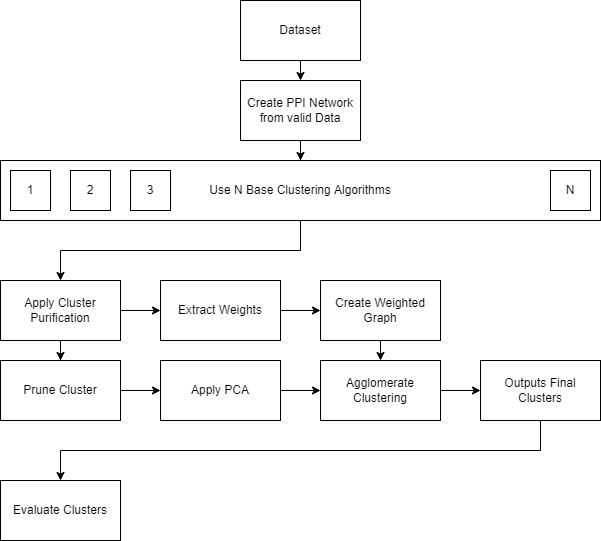
\includegraphics[width=0.15\textwidth]{images/systemdiag.png}
        \end{tikzfigure}
    }
    \column{0.25}
    \block[ bodyoffsety=2cm,
  titleoffsety=2cm]{Dataset}
    {
        PPI network datasets used for the purpose of this research have been extracted from primary sources such as BioGrid, MINT and Mentha as well as secondary or predictive databases such as String and primarily focus on a selected few species such as humans, mice, rats and yeast. The extraction process works by first collecting all possible proteins and their gene names for our selected species and then running queries for the extraction of PPI datasets for the respective proteins on online repositories. The datasets are then stored in a seperate database which contains a list of proteins and their interactions.
    }
 
    \block[bodyoffsety=2cm, titleoffsety=2cm]
    {Methodology}{
       Ensemble clustering is a promising method for protein complex identification problem. It relies on the use of $N$ number of base clustering algorithms which output a set of clusters for each algorithm.
       These different sets of clusters then go through the cluster purification stage where inconsistent clusters are discarded. Then dimensionality reduction is done through principal component analysis (PCA) in order to proceed to the final stage which is consensus clustering where the final clusters are obtained. 
       Our proposed method incorporates both biological and topological information in order to achieve more accurate results and to expand the list of features upon which complex prediction takes place. An overview of our pipeline can be seen on the left.
    }

  \column{0.25}
      
    \block[bodyoffsety=2cm, titleoffsety=2cm]
    {Clique Percolation}{

    }
   
    \block[ bodyoffsety=2cm,
  titleoffsety=2cm]{Genetic Algorithm}{
   The genetic algorithm (GA) is a bio-inspired meta-heuristic algorithm that tends to find better approximate solutions to NP-complete problems. The general steps of a GA are: initialize population randomly, while looping: evaluate fitness, select parents, create offspring through crossover \& mutation, update population. We initialize our population randomly and our fitness function is: \[
JD_{cut} (C1,\dots, C_k) = \sum_{k} \frac{W_{kk}}{A_k + W_{ki}} 
\]
Because of the volatile nature of the solutions, we do not use crossover to generate offspring. We only mutate selected parents to achieve variability in our solution space.
  }
  
  
  \block[ bodyoffsety=2cm,
  titleoffsety=2cm]{Graph Neural Networks}{
    
  }

  \block[ bodyoffsety=2cm,
  titleoffsety=2cm]{Consensus Algorithm}{
    
  }
  \block[ bodyoffsety=2cm,
  titleoffsety=2cm]{Predicting Predicted Protein Structure Function}{
    
  }

\column{0.25}
 \block[ bodyoffsety=2cm,
  titleoffsety=2cm]{Novelty}{ % Novelty factor is the 

  }
    \block[ bodyoffsety=2cm,
  titleoffsety=2cm]{Results}{ % Talk about how results will be achieved, what they will be, what they will signify

  }
  
  
  \block[ bodyoffsety=2cm,
  titleoffsety=2cm]{Conclusion}{ % Conclusion of the idea is pending
  }


\end{columns}
\end{document}
